

\section{学术要旨}
玄学是对道家的表达 .可以说玄学是道家的一种分支或改进.

魏晋之际,玄学含义是指立言与行事两个方面,并多以立言玄妙,行事雅远为玄远旷达.“玄远”,指远离具体事物,专门讨论“超言绝象”的本体论问题.因此,浮虚、玄虚、玄远之学可通称之为玄学.玄学家又大多是当时的名士.主要代表人物有何晏、王弼、阮籍、嵇康、向秀、郭象等.它是在汉代儒学(经学)衰落的基础上;是由汉代道家思想、黄老之学演变发展而来的\cite{Figueredo:2009dg}.是汉末魏初的清谈直接演化的产物.

魏晋玄学指魏晋时期以老庄(或三玄)思想为骨架,从两汉繁琐的经学解放出来,企图调和“自然”与“名教”的一种特定的哲学思潮.它讨论的中心问题是“本末有无”问题,即用思辨的方法讨论关于天地万物存在的根据的问题,也就是说它一种远离“事物”与“事务”的形式来讨论事务存在根据的本体论形而上学的问题.它是中国哲学史上第一次企图使中国哲学在老庄思想基础上建构把儒道两大家结合起来极有意义的哲学尝试. 在哲学上﹐主要以有无问题为中心﹐形成玄学的贵无与崇有两派.

\begin{table}[hbt]
	\caption{这是一张无聊的表}
	\centering
	\begin{tabular}{llr}
		\toprule
		\multicolumn{2}{c}{姓名} \\
		\cmidrule(r){1-2}
		名名名名名名 & 姓姓姓姓姓姓 & 分数 \\
		\midrule
		雷 & 张 &~$7.5$~\\
		梅梅 & 王 &~$2$~\\
		\bottomrule
	\end{tabular}
	\label{tab:label}
\end{table}

\section{简要介绍}


\subsection{释义}

玄学, 中国魏晋时期出现的一种崇尚老庄的思潮,一般特指魏晋玄学.“玄”这一概念,最早见于老子:
“玄之又玄,众妙之门.”王弼老子指略说:“玄,谓之深者也”.玄学即是研究幽深玄远问题的学说.

玄学又称新道家,是对老子、庄子和周易的研究和解说,产生于魏晋时期.玄学是中国魏晋时期到宋朝中叶之间出现的一种崇尚老庄的思潮.也可以说是道家之学以一种新的表现方式,故又有新道家之称.其思潮持续时间自汉末起至宋朝中叶结束.与世俗所谓玄学、玄虚实有不同.“玄”这一概念,最早出现于老子:“玄之又玄,众妙之门.”扬雄也讲玄,他在太玄?玄摛说:“玄者,幽摛万类,不见形者也.”王弼老子指略说:“玄,谓之深者也.”玄学即是研究幽深玄远问题的学说.魏晋时人注重老子、庄子和周易,称之为“三玄”,而老子、
庄子则被视为“玄宗”.魏晋玄学的主要代表人物有何晏、王弼、阮籍、嵇康、向秀、郭象等.

玄学之“玄”,出自老子的思想,老子·一章中说:“玄之又玄,众妙之门”.玄就是总天地万物的一般规律“道”,它体现了万物无穷奥妙的变化作用.玄学家们还用他们的老、庄思想来注解儒家的论语、
周易,对已经失去维系人心作用的两汉经学作了改造,建立起了“以无为本”的哲学本体论.儒家的“礼法”、“名教”、“人道”等思想,虽然也是玄学所讨论的内容,但其主旨却是道家的,即强调崇高的是“无”、“自然”和“无为”.

玄学所探讨的中心问题尽管仍可归结为天人关系问题,但在形式上,它已经摆脱了两汉经学章句笺注的繁琐破碎;在内容上,则抛弃了经学思潮的“天人感应”的粗俗的目的论之论证. 玄学家在多方面论证了道家的“自然”与儒家的“名教”二者是一致的,他们一改汉代“儒道互黜”的思想格局,主张“祖述老庄”,以道家为主调和儒道.玄学所提出的或着重关注的有无、本末、体用、言意、一多、动静、梦觉、本迹、自然与名教等一系列具有思辨性质的概念范畴都是道家所具备重视,而原始儒学和两汉经学所不具备或不重视的,玄学的出现大大推动了中国哲学的发展.

郎擎霄庄子学案概述说:当时达官名士,多宗老庄如魏王弼,、何晏、山涛、阮籍、嵇康、向秀、郭象,晋王济、王衍、卢谌、庾数、庾亮、桓石秀、司马彪、崔馔、李颐,宋戴顺、李叔乏、齐祖冲之、徐白珍,梁江轿、伏曼客、掼埸、严植之、刘昭、庾曼倩,陈周弘正、徐陵、全缓、张讥、陆瑜,北魏程骏、邱晏,北齐杜弼其最著者也.这是一个不小的名单,但并非全部.社会各阶层习庄之风蔚为大观,按吕思勉先生的说法,此风一直到隋才慢慢停息.“帝王、贵戚、大臣、武夫、儒生、文人、艺士、妇女无不能之.余风又流衍于北.入隋乃息\footnote{这是一个厉害的脚注} .”

玄学至东晋后不减反增更是风行,王弼周易注在南朝立于学官,南朝宋齐两代的官方四学都包括玄学,梁、陈两代又盛行讲论“三玄”之风,故而东晋南朝都应当是玄学的流行期.关于唐代的学术,过去人们都说是兼行儒释道三教.现在看来,唐朝的官方学术与民间学术应有不同,官方学术包括经学与道学,经学即五经及论语、孝经之学,其中周易用王弼注,论语用何晏的集解,这完全是玄学中易学的延续;唐代道学、道举尊崇老子、列子、文子、庄子四部书,四部书都称为经,这种道学可说是玄学中的老庄学的发扬或放大\footnote{这是另一个厉害的脚注}  .

通常意义上说,一个时代思潮在宏盛过后便会日渐式微,即使留些余绪,也不过气若游丝.而玄学思潮经历几百年的绵延,入唐后非但没有衰退,反而取得新一轮发展的恢弘气势.玄学至宋朝中叶被宋明理学取代.\cite{bollag2010clinical}

\subsection{演变}

东汉末年至两晋,是两百多年的乱世,随着东汉大一统王朝的分崩离析,统治思想界近四百年的儒家之学也开始失去了魅力,士大夫对两汉经学的繁琐学风、谶纬神学的怪诞浅薄,以及三纲五常的陈词滥调普遍感到厌倦,于是转而寻找新的"安身立命"之地,醉心于形而上的哲学论辩.这种论辩犹如后代的沙龙,风雅名士(以嵇康、阮籍为代表赫赫有名的"竹林七贤"恰是魏晋风度的化身),聚在一起,谈论玄道,当时人称之为"清谈"或"玄谈".

\begin{figure}[ht]
	\centering
	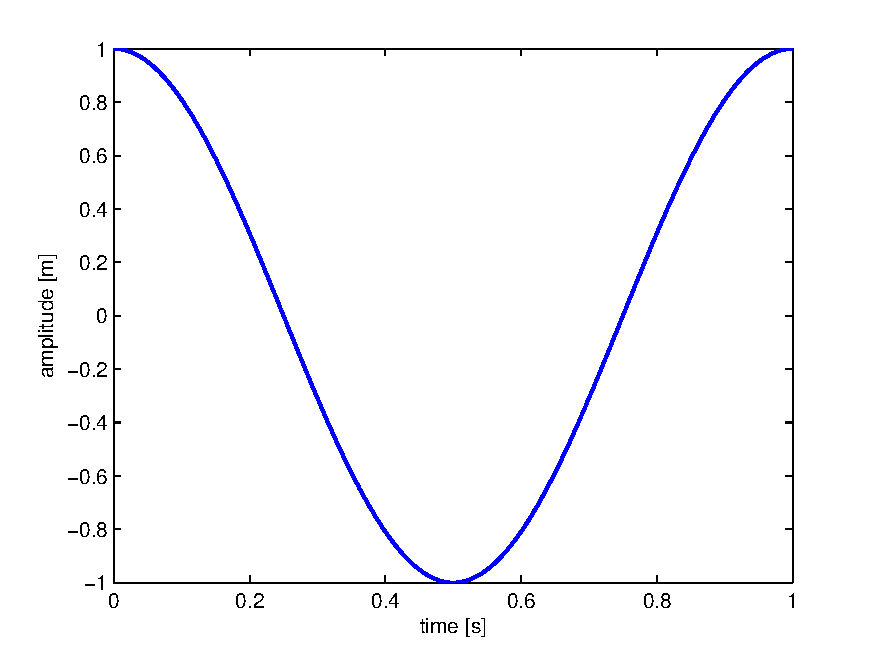
\includegraphics[width=\linewidth]{pic/results}
	\caption{这是一张图}
	\label{fig:results}
\end{figure}

玄学至东晋后不减反增更是风行,王弼周易注在南朝立于学官,南朝宋齐两代的官方四学都包括玄学,梁、陈两代又盛行讲论“三玄”之风,故而东晋南朝都应当是玄学的流行期.关于唐代的学术,过去人们都说是兼行儒释道三教.现在看来,唐朝的官方学术与民间学术应有不同,官方学术包括经学与道学,经学即五经及论语、孝经之学,其中周易用王弼注,论语用何晏的集解,这完全是玄学中易学的延续;唐代道学、道举尊崇老子、列子、文子、庄子四部书,四部书都称为经,这种道学可说是玄学中的老庄学的发扬或放大[2]  .玄学至宋朝中叶被宋明理学取代.

据清代学者赵翼二十二史剳记称,清谈之风始于魏齐王曹芳正始年间,何晏、王弼可以说是创始人,他们都是当时贵族名士,影响所及,便成一代风气.晋书上所谓"正始之音"也正是指整个魏晋时期玄谈风气.

何晏、王弼主张"贵无论",说"天地万物皆以无为本"(晋书·王衍传),又提出"名教"出于"自然"说.其后阮籍、嵇康主张"越名教任自然"(与山巨源绝交书).嵇康并"以六经为芜秽,以仁义为臭腐"(难自然好学论),"非汤武而薄周孔"(此句也是出自与山巨源绝交书,此篇文采斐然权不谈,一般来说可以算是嵇康的宣言书,甚至是当时魏晋二三子的宣言书,但窃以为,依当时历史情势来看,嵇康其意并非真的"越名教任自然,非汤武而薄周孔",而是作文明志而已,说地明白点,便是让那司马家知道自己的心思,而事实上显然不是真的坚决"越名教任自然,非汤武而薄周孔",这在嵇康其它文章中可知一斑).其后完成于郭象,其作庄子注,此书一出,玄学大畅,"儒墨之迹见鄙,道家之言遂盛焉"(晋书·郭象传).

\begin{equation}\label{key}
\sum_{n=1}^{\infty} \dfrac{1}{n^2} = \dfrac{\pi^2}{6}.
\end{equation}

从嵇康、阮籍、张湛、韩伯、陶渊明、袁宏等玄学家的思想可以看出,如果说,魏晋玄学是精致的形而上的哲理玄思,则当时的养生可谓是实践中的操作,这二者,构成了互为表里的关系.对此,汤用彤早已指出:“中华方术与玄学既俱本乎道家自然之说.汉魏之际,清谈之风大盛,佛经之译出较多,于是佛教乃脱离方术而独立,进而高谈清净无为之玄致.其中演变之关键有二要义,一日佛,一目道.

\begin{equation}\label{key}
\sum_{n=1}^{\infty} \dfrac{1}{n^4} = \dfrac{\pi^4}{90}.
\end{equation}




由此二义,变迁附益,至魏晋之世遂进为玄理之大宗也~0”牟宗三先生也说过:“道家工夫自心上作,而在性上收获.无论是‘不离于宗’之天人,或不离于精不离于真之至人、神人,皆是从心上作致虚守静之工夫.从此作虚静浑化之玄冥工夫,始至天人、至人、神人之境,而养生之义亦摄于其中矣.”这一论断甚为精透.道家本体的实体性、实在性,透过养生、长生说即可转化为神仙术.他又说:“通过修炼之工夫而至长生,成仙,则是顺道家而来之道教,已发于第二义.